\documentclass[border=1pt]{standalone}
\usepackage[dvipsnames]{xcolor}
\usepackage{tikz}                       % Graphen und kommutative Diagramme
\usetikzlibrary{patterns}               % Um schraffierte Formen in der tikzpicture-Umgebung zu zeichnen.
\newcommand{\ul}[1]{\underline{\smash{#1}}}

\begin{document}
\centering
\begin{minipage}{.5\textwidth}
\centering
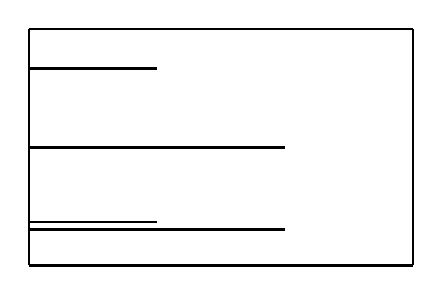
\begin{tikzpicture}[yscale=.8, xscale=1.3, x=1.25cm, y=1.25cm, line width=1pt]
    \draw (0,0.5) -- (3,0.5);
    \draw (0,3.5) -- (3,3.5);
    \draw (0,0.5) -- (0,3.5);
    \draw (3,0.5) -- (3,3.5);
    
    \draw[line width=1pt] (0,3) to (1,3);
    \draw[line width=1pt] (0,1.05) to (1,1.05);
    
    \draw[line width=1pt] (0,2) to (2,2);
    \draw[line width=1pt] (0,0.95) to (2,0.95);
\end{tikzpicture}
\end{minipage}
\end{document}
